%% Author_tex.tex
%% V1.0
%% 2012/13/12
%% developed by Techset
%%
%% This file describes the coding for rsproca.cls

\documentclass[]{rsos}%%%%where rsos is the template name

\usepackage{lineno}
\linenumbers

\usepackage[T1]{fontenc}
\usepackage[utf8]{inputenc}


% tightlist command for lists without linebreak
\providecommand{\tightlist}{%
  \setlength{\itemsep}{0pt}\setlength{\parskip}{0pt}}

% From pandoc table feature
\usepackage{longtable,booktabs,array}
\usepackage{calc} % for calculating minipage widths
% Correct order of tables after \paragraph or \subparagraph
\usepackage{etoolbox}
\makeatletter
\patchcmd\longtable{\par}{\if@noskipsec\mbox{}\fi\par}{}{}
\makeatother
% Allow footnotes in longtable head/foot
\IfFileExists{footnotehyper.sty}{\usepackage{footnotehyper}}{\usepackage{footnote}}
\makesavenoteenv{longtable}



%%%% *** Do not adjust lengths that control margins, column widths, etc. ***

%%%%%%%%%%% Defining Enunciations  %%%%%%%%%%%
\newtheorem{theorem}{\bf Theorem}[section]
\newtheorem{condition}{\bf Condition}[section]
\newtheorem{corollary}{\bf Corollary}[section]
%%%%%%%%%%%%%%%%%%%%%%%%%%%%%%%%%%%%%%%%%%%%%%%

\begin{document}


%%%% Article title to be placed here
\title{Institutional affiliations of editors in ecology, evolution, and conservation}

\author{
Emilio M. Bruna$^{1,2}$,
Author Two$^{1}$}

\address{
  $^{1}$Department of Wildlife Ecology and Conservation, University of Florida, PO Box 110430, Gainesville, Florida, 32611 USA\\
  $^{2}$Center for Latin American Studies, University of Florida, PO Box 110530, Gainesville, Florida, 32611-0530 USA}
%%%% Subject entries to be placed here %%%%
\subject{
Science, society \& policy}

%%%% Keyword entries to be placed here %%%%
\keywords{
Editorial boards,
Implicit bias,
Global North,
Global South}

%%%% Insert corresponding author and its email address}
\corres{
  E. M. Bruna\\
  e-mail: \href{mailto:embruna@ufl.edu}{\nolinkurl{embruna@ufl.edu}}
}

%%%% Abstract text to be placed here %%%%%%%%%%%%
\begin{abstract}
The abstract text goes here. The abstract text goes here. The abstract text goes here. The abstract text goes here. The abstract text goes here. The abstract text goes here. The abstract text goes here. The abstract text goes here.
\end{abstract}
%%%%%%%%%%%%%%%%%%%%%%%%%%%

\providecommand{\EndFirstPage}{%
}

\begin{fmtext}

\hypertarget{introduction}{%
\section{Introduction}\label{introduction}}

p1: institutional affiliation matters in publishing, which is a critical element of professional advancement. Work in fields like econ has shown that\ldots{}

\citep{addisEditorialBoardsItalian2003}
\citep{hodgsonEditorsAuthorsEconomics1999}
p2: documenting institutional affiliations is an essential first step is assessing the potential for such impacts. Studies documenting such affiliations are rare in the natural sciences. Furthermore, most studies take a relatively short ``snapshot'', which makes it impossible to evaluate potential temporal trends in relation to increased awareness and the global expansion of the scholarship.

p3: What is known about editorial boards of EEC journals We used data on the institutional affiliations of over XXXX scientists to test the prediction that (i) the editorial boards of journals in ecology, evolution, and conservation would exhibit patterns of institutional dominance similar to those observed in other fields, but that (ii) this dominance would decrease overtime. However, we also predicted that (iii) increases in the institutional diversity of editorial boards would result from adding novel institutions in Europe and North America, and not from adding editors based at institutions in the Global South.

\end{fmtext}
\maketitle

\hypertarget{methods}{%
\section{Methods}\label{methods}}

\hypertarget{data-collection}{%
\subsection{Data Collection}\label{data-collection}}

Subsection text here.

\hypertarget{additional-subsection-if-necessary}{%
\subsubsection{Additional Subsection if necessary}\label{additional-subsection-if-necessary}}

\hypertarget{analysis}{%
\subsection{Analysis}\label{analysis}}

\hypertarget{results}{%
\section{Results}\label{results}}

\hypertarget{institutional-dominance}{%
\subsection{Institutional dominance}\label{institutional-dominance}}

\hypertarget{temporal-trends}{%
\subsection{Temporal trends}\label{temporal-trends}}

\hypertarget{discussion}{%
\section{Discussion}\label{discussion}}

\hypertarget{temporal-patterns}{%
\subsection{Temporal Patterns}\label{temporal-patterns}}

Subsubsection text here.

Line 1

Line 2

Line 3

Line 4

Line 5

Line 6

Line 7

Line 8

Line 9

Line 10

Line 11

Line 12

Line 13

Line 14

Line 15

Line 16

Line 17

Line 18

Line 19

\EndFirstPage

\hypertarget{lists}{%
\section{Lists}\label{lists}}

\begin{itemize}
\item
  one
\item
  two
\item
  three
\item
  fruits

  \begin{itemize}
  \tightlist
  \item
    apples

    \begin{itemize}
    \tightlist
    \item
      macintosh
    \item
      red delicious
    \end{itemize}
  \item
    pears
  \item
    peaches
  \end{itemize}
\item
  vegetables

  \begin{itemize}
  \tightlist
  \item
    broccoli
  \item
    chard
  \end{itemize}
\end{itemize}

\hypertarget{citations}{%
\subsection{Citations}\label{citations}}

Blabla \cite{Lannes} blabla. Blabla \cite{HJ2} blabla. Blabla \cite{BF, Lannes} blabla. Blabla \cite{Benjamin1967, HJ2, HJ3, HP2} blabla.

\begin{figure}

{\centering 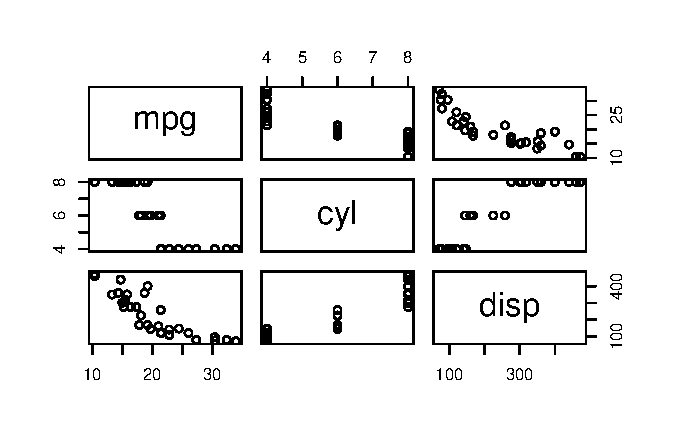
\includegraphics{Bruna_etal_MS_files/figure-latex/nice-plot-1} 

}

\caption{The caption}\label{fig:nice-plot}
\end{figure}

\ethics{Please provide details on the ethics.}

\dataccess{Data used in this manuscript are archived at the Dryad Digital Repository (\emph{url added upon acceptance}). Code used for analyses and to generate figures is archived Zenodo (\emph{url added upon acceptance}) with updates available at Github.}

\aucontribute{Contributorship roles (e.g., CRediT, \url{https://casrai.org/credit/}):\\
EMB: Conceptualization,Methodology, Investigation, Formal analysis, Data curation, Visualization, Writing - Original Draft Preparation, Writing - Review \& Editing, Project administration, Supervision}

\competing{Bruna was Editor-in-Chief of \emph{Biotropica} from 2013-2019 and is currently the Secretary of the Ecological Society of America, which publishes the journal \emph{Ecology}. None of the other autors have any conflicts-of-interest to declare.}

\funding{This project was supported by grants from the Mindlin Foundation, the UF Center for Latin American Studies, and the UF Informatics Institute.}


\ack{The authors thank -- --, -- --, and -- -- for their feedback on drafts of the manuscript and assistance with data collection.}

\bibliographystyle{RS}
\bibliography{refs.bib}


\end{document}
